\chapter{Simultaneous viewing of images and surfaces}

Images and surfaces can be viewed simultaneously by \textbf{left-clicking} on the shortcut (Figure~\ref{fig:slice_plane_original}) located in the lower right corner of the InVesalius interface.

\begin{figure}[!htb]
\centering

\includegraphics[scale=0.6]{slice_plane_original}
\caption{Shortcut for simultaneous viewing}
\label{fig:slice_plane_original}
\end{figure}

This feature allows users to enable or disable the displaying of images in different orientations (or plans) within the same display window of the 3D surface. Simply check or uncheck the corresponding option in the menu shown in Figure~\ref{fig:view_2d_3d_1}.

\begin{figure}[!htb]
\centering
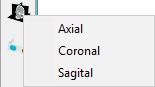
\includegraphics[scale=0.6]{view_2d_3d_1_en.png}
\caption{Selection of the guidelines (plans) to display}
\label{fig:view_2d_3d_1}
\end{figure}

It is worth noting that when a particular orientation is selected, a check is presented in the corresponding option. This is illustrated in Figure~\ref{fig:view_2d_3d_2}.

\begin{figure}[!htb]
\centering
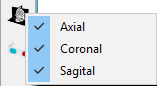
\includegraphics[scale=0.6]{view_2d_3d_2_en.png}
\caption{Selected Guidelines for display}
\label{fig:view_2d_3d_2}
\end{figure}

\newpage

If the surface is already displayed, the plans of the guidelines will be presented as shown in Figure~\ref{fig:only_2d_planes}. Otherwise, only the plans will be displayed.

\begin{figure}[!htb]
\centering
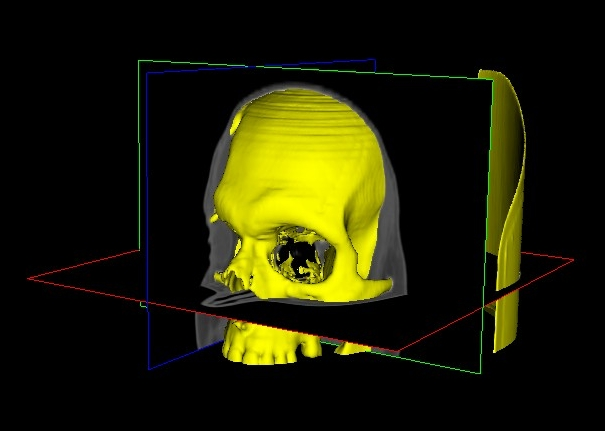
\includegraphics[scale=0.5]{3d_planes}
\caption{Surface and plans displayed simultaneously}
\label{fig:3d_planes}
\end{figure}

\begin{figure}[!htb]
\centering
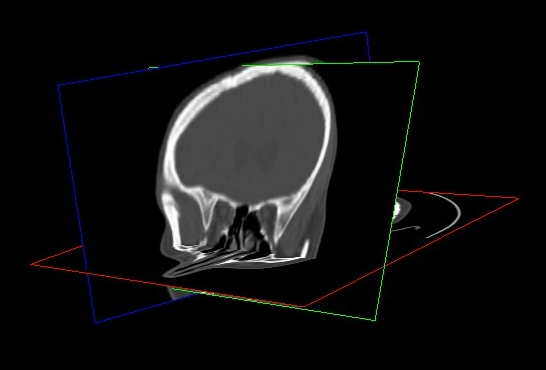
\includegraphics[scale=0.55]{only_2d_planes}
\caption{Flat display (no surface)}
\label{fig:only_2d_planes}
\end{figure}

\newpage

To view the display of a plan, just uncheck the corresponding option in the menu (Figure~\ref{fig:view_2d_3d_2}).